% Created by tikzDevice version 0.12.6 on 2024-06-11 19:56:44
% !TEX encoding = UTF-8 Unicode
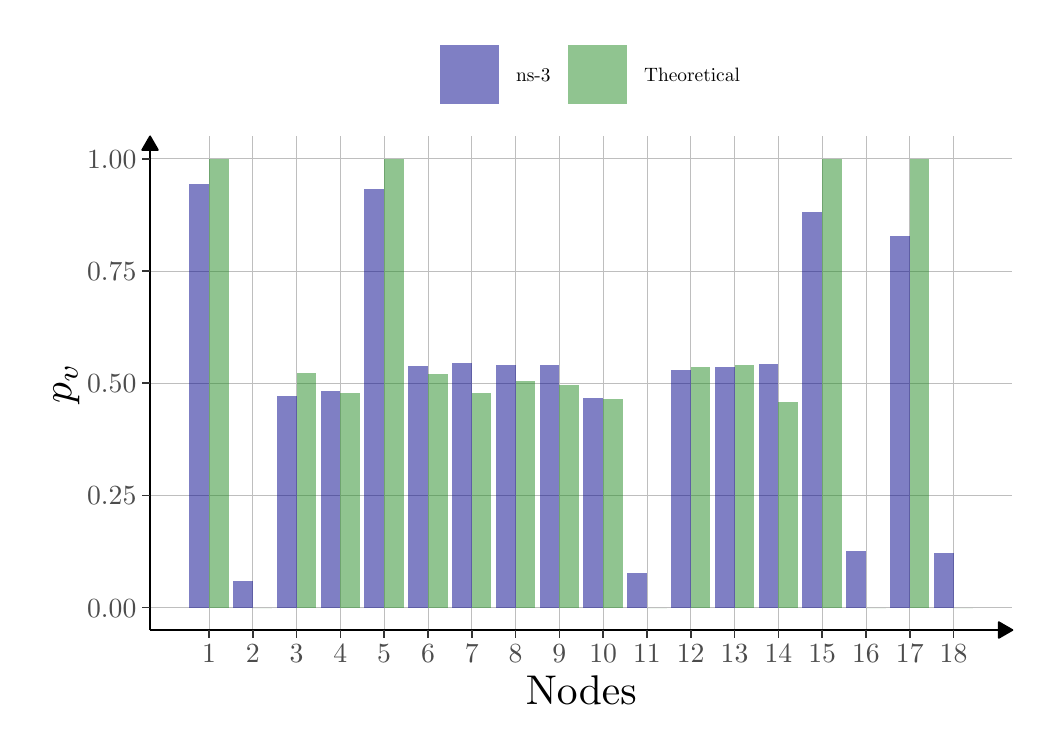
\begin{tikzpicture}[x=1pt,y=1pt]
\definecolor{fillColor}{RGB}{255,255,255}
\path[use as bounding box,fill=fillColor,fill opacity=0.00] (0,0) rectangle (361.35,252.94);
\begin{scope}
\path[clip] (  0.00,  0.00) rectangle (361.35,252.94);
\definecolor{drawColor}{RGB}{255,255,255}
\definecolor{fillColor}{RGB}{255,255,255}

\path[draw=drawColor,line width= 0.6pt,line join=round,line cap=round,fill=fillColor] (  0.00,  0.00) rectangle (361.35,252.94);
\end{scope}
\begin{scope}
\path[clip] ( 44.22, 35.28) rectangle (355.85,213.68);
\definecolor{fillColor}{RGB}{255,255,255}

\path[fill=fillColor] ( 44.22, 35.28) rectangle (355.85,213.68);
\definecolor{drawColor}{RGB}{190,190,190}

\path[draw=drawColor,line width= 0.3pt,line join=round] ( 44.22, 43.39) --
	(355.85, 43.39);

\path[draw=drawColor,line width= 0.3pt,line join=round] ( 44.22, 83.93) --
	(355.85, 83.93);

\path[draw=drawColor,line width= 0.3pt,line join=round] ( 44.22,124.48) --
	(355.85,124.48);

\path[draw=drawColor,line width= 0.3pt,line join=round] ( 44.22,165.03) --
	(355.85,165.03);

\path[draw=drawColor,line width= 0.3pt,line join=round] ( 44.22,205.57) --
	(355.85,205.57);

\path[draw=drawColor,line width= 0.3pt,line join=round] ( 65.51, 35.28) --
	( 65.51,213.68);

\path[draw=drawColor,line width= 0.3pt,line join=round] ( 81.33, 35.28) --
	( 81.33,213.68);

\path[draw=drawColor,line width= 0.3pt,line join=round] ( 97.16, 35.28) --
	( 97.16,213.68);

\path[draw=drawColor,line width= 0.3pt,line join=round] (112.99, 35.28) --
	(112.99,213.68);

\path[draw=drawColor,line width= 0.3pt,line join=round] (128.81, 35.28) --
	(128.81,213.68);

\path[draw=drawColor,line width= 0.3pt,line join=round] (144.64, 35.28) --
	(144.64,213.68);

\path[draw=drawColor,line width= 0.3pt,line join=round] (160.47, 35.28) --
	(160.47,213.68);

\path[draw=drawColor,line width= 0.3pt,line join=round] (176.29, 35.28) --
	(176.29,213.68);

\path[draw=drawColor,line width= 0.3pt,line join=round] (192.12, 35.28) --
	(192.12,213.68);

\path[draw=drawColor,line width= 0.3pt,line join=round] (207.95, 35.28) --
	(207.95,213.68);

\path[draw=drawColor,line width= 0.3pt,line join=round] (223.78, 35.28) --
	(223.78,213.68);

\path[draw=drawColor,line width= 0.3pt,line join=round] (239.60, 35.28) --
	(239.60,213.68);

\path[draw=drawColor,line width= 0.3pt,line join=round] (255.43, 35.28) --
	(255.43,213.68);

\path[draw=drawColor,line width= 0.3pt,line join=round] (271.26, 35.28) --
	(271.26,213.68);

\path[draw=drawColor,line width= 0.3pt,line join=round] (287.08, 35.28) --
	(287.08,213.68);

\path[draw=drawColor,line width= 0.3pt,line join=round] (302.91, 35.28) --
	(302.91,213.68);

\path[draw=drawColor,line width= 0.3pt,line join=round] (318.74, 35.28) --
	(318.74,213.68);

\path[draw=drawColor,line width= 0.3pt,line join=round] (334.56, 35.28) --
	(334.56,213.68);
\definecolor{fillColor}{RGB}{0,0,139}

\path[fill=fillColor,fill opacity=0.50] ( 58.39, 43.39) rectangle ( 65.51,196.31);
\definecolor{fillColor}{RGB}{34,139,34}

\path[fill=fillColor,fill opacity=0.50] ( 65.51, 43.39) rectangle ( 72.63,205.57);

\path[fill=fillColor,fill opacity=0.50] ( 81.33, 43.39) rectangle ( 88.46, 43.39);
\definecolor{fillColor}{RGB}{0,0,139}

\path[fill=fillColor,fill opacity=0.50] ( 74.21, 43.39) rectangle ( 81.33, 53.07);

\path[fill=fillColor,fill opacity=0.50] ( 90.04, 43.39) rectangle ( 97.16,119.72);
\definecolor{fillColor}{RGB}{34,139,34}

\path[fill=fillColor,fill opacity=0.50] ( 97.16, 43.39) rectangle (104.28,128.05);

\path[fill=fillColor,fill opacity=0.50] (112.99, 43.39) rectangle (120.11,120.75);
\definecolor{fillColor}{RGB}{0,0,139}

\path[fill=fillColor,fill opacity=0.50] (105.87, 43.39) rectangle (112.99,121.58);

\path[fill=fillColor,fill opacity=0.50] (121.69, 43.39) rectangle (128.81,194.69);
\definecolor{fillColor}{RGB}{34,139,34}

\path[fill=fillColor,fill opacity=0.50] (128.81, 43.39) rectangle (135.94,205.57);

\path[fill=fillColor,fill opacity=0.50] (144.64, 43.39) rectangle (151.76,127.72);
\definecolor{fillColor}{RGB}{0,0,139}

\path[fill=fillColor,fill opacity=0.50] (137.52, 43.39) rectangle (144.64,130.80);
\definecolor{fillColor}{RGB}{34,139,34}

\path[fill=fillColor,fill opacity=0.50] (160.47, 43.39) rectangle (167.59,121.07);
\definecolor{fillColor}{RGB}{0,0,139}

\path[fill=fillColor,fill opacity=0.50] (153.35, 43.39) rectangle (160.47,131.71);
\definecolor{fillColor}{RGB}{34,139,34}

\path[fill=fillColor,fill opacity=0.50] (176.29, 43.39) rectangle (183.42,125.13);
\definecolor{fillColor}{RGB}{0,0,139}

\path[fill=fillColor,fill opacity=0.50] (169.17, 43.39) rectangle (176.29,130.97);
\definecolor{fillColor}{RGB}{34,139,34}

\path[fill=fillColor,fill opacity=0.50] (192.12, 43.39) rectangle (199.24,123.83);
\definecolor{fillColor}{RGB}{0,0,139}

\path[fill=fillColor,fill opacity=0.50] (185.00, 43.39) rectangle (192.12,130.97);
\definecolor{fillColor}{RGB}{34,139,34}

\path[fill=fillColor,fill opacity=0.50] (207.95, 43.39) rectangle (215.07,118.64);
\definecolor{fillColor}{RGB}{0,0,139}

\path[fill=fillColor,fill opacity=0.50] (200.83, 43.39) rectangle (207.95,119.02);
\definecolor{fillColor}{RGB}{34,139,34}

\path[fill=fillColor,fill opacity=0.50] (223.78, 43.39) rectangle (230.90, 43.39);
\definecolor{fillColor}{RGB}{0,0,139}

\path[fill=fillColor,fill opacity=0.50] (216.65, 43.39) rectangle (223.78, 55.81);

\path[fill=fillColor,fill opacity=0.50] (232.48, 43.39) rectangle (239.60,129.10);
\definecolor{fillColor}{RGB}{34,139,34}

\path[fill=fillColor,fill opacity=0.50] (239.60, 43.39) rectangle (246.72,130.16);
\definecolor{fillColor}{RGB}{0,0,139}

\path[fill=fillColor,fill opacity=0.50] (248.31, 43.39) rectangle (255.43,130.47);
\definecolor{fillColor}{RGB}{34,139,34}

\path[fill=fillColor,fill opacity=0.50] (255.43, 43.39) rectangle (262.55,131.13);

\path[fill=fillColor,fill opacity=0.50] (271.26, 43.39) rectangle (278.38,117.67);
\definecolor{fillColor}{RGB}{0,0,139}

\path[fill=fillColor,fill opacity=0.50] (264.13, 43.39) rectangle (271.26,131.24);

\path[fill=fillColor,fill opacity=0.50] (279.96, 43.39) rectangle (287.08,186.47);
\definecolor{fillColor}{RGB}{34,139,34}

\path[fill=fillColor,fill opacity=0.50] (287.08, 43.39) rectangle (294.20,205.57);

\path[fill=fillColor,fill opacity=0.50] (302.91, 43.39) rectangle (310.03, 43.39);
\definecolor{fillColor}{RGB}{0,0,139}

\path[fill=fillColor,fill opacity=0.50] (295.79, 43.39) rectangle (302.91, 63.86);

\path[fill=fillColor,fill opacity=0.50] (311.61, 43.39) rectangle (318.74,177.60);
\definecolor{fillColor}{RGB}{34,139,34}

\path[fill=fillColor,fill opacity=0.50] (318.74, 43.39) rectangle (325.86,205.57);

\path[fill=fillColor,fill opacity=0.50] (334.56, 43.39) rectangle (341.69, 43.39);
\definecolor{fillColor}{RGB}{0,0,139}

\path[fill=fillColor,fill opacity=0.50] (327.44, 43.39) rectangle (334.56, 63.18);
\end{scope}
\begin{scope}
\path[clip] (  0.00,  0.00) rectangle (361.35,252.94);
\definecolor{drawColor}{RGB}{0,0,0}

\path[draw=drawColor,line width= 0.6pt,line join=round] ( 44.22, 35.28) --
	( 44.22,213.68);
\definecolor{fillColor}{RGB}{0,0,0}

\path[draw=drawColor,line width= 0.6pt,line join=round,fill=fillColor] ( 47.07,208.75) --
	( 44.22,213.68) --
	( 41.37,208.75) --
	cycle;
\end{scope}
\begin{scope}
\path[clip] (  0.00,  0.00) rectangle (361.35,252.94);
\definecolor{drawColor}{gray}{0.30}

\node[text=drawColor,anchor=base east,inner sep=0pt, outer sep=0pt, scale=  1.00] at ( 39.27, 39.94) {0.00};

\node[text=drawColor,anchor=base east,inner sep=0pt, outer sep=0pt, scale=  1.00] at ( 39.27, 80.49) {0.25};

\node[text=drawColor,anchor=base east,inner sep=0pt, outer sep=0pt, scale=  1.00] at ( 39.27,121.04) {0.50};

\node[text=drawColor,anchor=base east,inner sep=0pt, outer sep=0pt, scale=  1.00] at ( 39.27,161.58) {0.75};

\node[text=drawColor,anchor=base east,inner sep=0pt, outer sep=0pt, scale=  1.00] at ( 39.27,202.13) {1.00};
\end{scope}
\begin{scope}
\path[clip] (  0.00,  0.00) rectangle (361.35,252.94);
\definecolor{drawColor}{gray}{0.20}

\path[draw=drawColor,line width= 0.6pt,line join=round] ( 41.47, 43.39) --
	( 44.22, 43.39);

\path[draw=drawColor,line width= 0.6pt,line join=round] ( 41.47, 83.93) --
	( 44.22, 83.93);

\path[draw=drawColor,line width= 0.6pt,line join=round] ( 41.47,124.48) --
	( 44.22,124.48);

\path[draw=drawColor,line width= 0.6pt,line join=round] ( 41.47,165.03) --
	( 44.22,165.03);

\path[draw=drawColor,line width= 0.6pt,line join=round] ( 41.47,205.57) --
	( 44.22,205.57);
\end{scope}
\begin{scope}
\path[clip] (  0.00,  0.00) rectangle (361.35,252.94);
\definecolor{drawColor}{RGB}{0,0,0}

\path[draw=drawColor,line width= 0.6pt,line join=round] ( 44.22, 35.28) --
	(355.85, 35.28);
\definecolor{fillColor}{RGB}{0,0,0}

\path[draw=drawColor,line width= 0.6pt,line join=round,fill=fillColor] (350.92, 32.43) --
	(355.85, 35.28) --
	(350.92, 38.12) --
	cycle;
\end{scope}
\begin{scope}
\path[clip] (  0.00,  0.00) rectangle (361.35,252.94);
\definecolor{drawColor}{gray}{0.20}

\path[draw=drawColor,line width= 0.6pt,line join=round] ( 65.51, 32.53) --
	( 65.51, 35.28);

\path[draw=drawColor,line width= 0.6pt,line join=round] ( 81.33, 32.53) --
	( 81.33, 35.28);

\path[draw=drawColor,line width= 0.6pt,line join=round] ( 97.16, 32.53) --
	( 97.16, 35.28);

\path[draw=drawColor,line width= 0.6pt,line join=round] (112.99, 32.53) --
	(112.99, 35.28);

\path[draw=drawColor,line width= 0.6pt,line join=round] (128.81, 32.53) --
	(128.81, 35.28);

\path[draw=drawColor,line width= 0.6pt,line join=round] (144.64, 32.53) --
	(144.64, 35.28);

\path[draw=drawColor,line width= 0.6pt,line join=round] (160.47, 32.53) --
	(160.47, 35.28);

\path[draw=drawColor,line width= 0.6pt,line join=round] (176.29, 32.53) --
	(176.29, 35.28);

\path[draw=drawColor,line width= 0.6pt,line join=round] (192.12, 32.53) --
	(192.12, 35.28);

\path[draw=drawColor,line width= 0.6pt,line join=round] (207.95, 32.53) --
	(207.95, 35.28);

\path[draw=drawColor,line width= 0.6pt,line join=round] (223.78, 32.53) --
	(223.78, 35.28);

\path[draw=drawColor,line width= 0.6pt,line join=round] (239.60, 32.53) --
	(239.60, 35.28);

\path[draw=drawColor,line width= 0.6pt,line join=round] (255.43, 32.53) --
	(255.43, 35.28);

\path[draw=drawColor,line width= 0.6pt,line join=round] (271.26, 32.53) --
	(271.26, 35.28);

\path[draw=drawColor,line width= 0.6pt,line join=round] (287.08, 32.53) --
	(287.08, 35.28);

\path[draw=drawColor,line width= 0.6pt,line join=round] (302.91, 32.53) --
	(302.91, 35.28);

\path[draw=drawColor,line width= 0.6pt,line join=round] (318.74, 32.53) --
	(318.74, 35.28);

\path[draw=drawColor,line width= 0.6pt,line join=round] (334.56, 32.53) --
	(334.56, 35.28);
\end{scope}
\begin{scope}
\path[clip] (  0.00,  0.00) rectangle (361.35,252.94);
\definecolor{drawColor}{gray}{0.30}

\node[text=drawColor,anchor=base,inner sep=0pt, outer sep=0pt, scale=  1.00] at ( 65.51, 23.44) {1};

\node[text=drawColor,anchor=base,inner sep=0pt, outer sep=0pt, scale=  1.00] at ( 81.33, 23.44) {2};

\node[text=drawColor,anchor=base,inner sep=0pt, outer sep=0pt, scale=  1.00] at ( 97.16, 23.44) {3};

\node[text=drawColor,anchor=base,inner sep=0pt, outer sep=0pt, scale=  1.00] at (112.99, 23.44) {4};

\node[text=drawColor,anchor=base,inner sep=0pt, outer sep=0pt, scale=  1.00] at (128.81, 23.44) {5};

\node[text=drawColor,anchor=base,inner sep=0pt, outer sep=0pt, scale=  1.00] at (144.64, 23.44) {6};

\node[text=drawColor,anchor=base,inner sep=0pt, outer sep=0pt, scale=  1.00] at (160.47, 23.44) {7};

\node[text=drawColor,anchor=base,inner sep=0pt, outer sep=0pt, scale=  1.00] at (176.29, 23.44) {8};

\node[text=drawColor,anchor=base,inner sep=0pt, outer sep=0pt, scale=  1.00] at (192.12, 23.44) {9};

\node[text=drawColor,anchor=base,inner sep=0pt, outer sep=0pt, scale=  1.00] at (207.95, 23.44) {10};

\node[text=drawColor,anchor=base,inner sep=0pt, outer sep=0pt, scale=  1.00] at (223.78, 23.44) {11};

\node[text=drawColor,anchor=base,inner sep=0pt, outer sep=0pt, scale=  1.00] at (239.60, 23.44) {12};

\node[text=drawColor,anchor=base,inner sep=0pt, outer sep=0pt, scale=  1.00] at (255.43, 23.44) {13};

\node[text=drawColor,anchor=base,inner sep=0pt, outer sep=0pt, scale=  1.00] at (271.26, 23.44) {14};

\node[text=drawColor,anchor=base,inner sep=0pt, outer sep=0pt, scale=  1.00] at (287.08, 23.44) {15};

\node[text=drawColor,anchor=base,inner sep=0pt, outer sep=0pt, scale=  1.00] at (302.91, 23.44) {16};

\node[text=drawColor,anchor=base,inner sep=0pt, outer sep=0pt, scale=  1.00] at (318.74, 23.44) {17};

\node[text=drawColor,anchor=base,inner sep=0pt, outer sep=0pt, scale=  1.00] at (334.56, 23.44) {18};
\end{scope}
\begin{scope}
\path[clip] (  0.00,  0.00) rectangle (361.35,252.94);
\definecolor{drawColor}{RGB}{0,0,0}

\node[text=drawColor,anchor=base,inner sep=0pt, outer sep=0pt, scale=  1.50] at (200.04,  8.42) {Nodes};
\end{scope}
\begin{scope}
\path[clip] (  0.00,  0.00) rectangle (361.35,252.94);
\definecolor{drawColor}{RGB}{0,0,0}

\node[text=drawColor,rotate= 90.00,anchor=base,inner sep=0pt, outer sep=0pt, scale=  1.50] at ( 15.83,124.48) {$p_v$};
\end{scope}
\begin{scope}
\path[clip] (  0.00,  0.00) rectangle (361.35,252.94);
\definecolor{fillColor}{RGB}{255,255,255}

\path[fill=fillColor] (142.72,224.68) rectangle (257.35,247.45);
\end{scope}
\begin{scope}
\path[clip] (  0.00,  0.00) rectangle (361.35,252.94);
\definecolor{fillColor}{RGB}{255,255,255}

\path[fill=fillColor] (148.22,224.68) rectangle (170.98,247.45);
\end{scope}
\begin{scope}
\path[clip] (  0.00,  0.00) rectangle (361.35,252.94);
\definecolor{fillColor}{RGB}{0,0,139}

\path[fill=fillColor,fill opacity=0.50] (148.93,225.39) rectangle (170.27,246.73);
\end{scope}
\begin{scope}
\path[clip] (  0.00,  0.00) rectangle (361.35,252.94);
\definecolor{fillColor}{RGB}{255,255,255}

\path[fill=fillColor] (194.46,224.68) rectangle (217.23,247.45);
\end{scope}
\begin{scope}
\path[clip] (  0.00,  0.00) rectangle (361.35,252.94);
\definecolor{fillColor}{RGB}{34,139,34}

\path[fill=fillColor,fill opacity=0.50] (195.18,225.39) rectangle (216.52,246.73);
\end{scope}
\begin{scope}
\path[clip] (  0.00,  0.00) rectangle (361.35,252.94);
\definecolor{drawColor}{RGB}{0,0,0}

\node[text=drawColor,anchor=base west,inner sep=0pt, outer sep=0pt, scale=  0.70] at (176.48,233.65) {ns-3};
\end{scope}
\begin{scope}
\path[clip] (  0.00,  0.00) rectangle (361.35,252.94);
\definecolor{drawColor}{RGB}{0,0,0}

\node[text=drawColor,anchor=base west,inner sep=0pt, outer sep=0pt, scale=  0.70] at (222.73,233.65) {Theoretical};
\end{scope}
\end{tikzpicture}
